\documentclass[11pt,a4paper]{article}

%\usepackage[utf8x]{inputenc}

\usepackage{mathpazo}
\usepackage{microtype}
\usepackage{verbatim}
\usepackage{url}

\usepackage{tikz}
\usetikzlibrary{intersections,calc,through,arrows.meta}
\tikzset{>=Stealth}

\textwidth=155mm
\textheight=230mm
\topmargin=0pt
\headheight=0pt
\oddsidemargin=0mm
\evensidemargin=0mm
\headsep=0pt
\parindent=0pt
\renewcommand{\baselinestretch}{1.15}
\setlength{\parskip}{0.3\baselineskip plus 1pt minus 1pt}

\setcounter{tocdepth}{1}

\newcommand*{\disfrac}[2]{\displaystyle\frac{#1}{#2}}
\newcommand*{\sm}[1]{$\scriptstyle #1$}

\newenvironment{form}[1]{%
\begin{displaymath}%
\renewcommand{\arraystretch}{#1}%
\begin{array}{lcl}}%
{\end{array}%
\end{displaymath}%
}

\begin{document}
\thispagestyle{empty}

\begin{center}
\textbf{\LARGE Lill's Method}

\bigskip
\bigskip

\textbf{\Large Moti Ben-Ari}

\bigskip
\bigskip

\url{http://www.weizmann.ac.il/sci-tea/benari/}


\bigskip
\bigskip

Version 0.2
\end{center}

\bigskip
\bigskip
\bigskip

\begin{small}
\begin{center}
\copyright{}\ 2020 Moti Ben-Ari
\end{center}

This work is licensed under the Creative Commons Attribution-ShareAlike 3.0 Unported License. To view a copy of this license, visit \url{http://creativecommons.org/licenses/by-sa/3.0/} or send a letter to Creative Commons, 444 Castro Street, Suite 900, Mountain View, California, 94041, USA.
\end{small}

\newpage

\section{Magic}\label{s.magic}

Construct a path consisting of four line segments $\{a_3,a_2,a_1,a_0\}$ of lengths:
\[
\{a_3=1,a_2=6,a_1=11,a_0=6\}\,,
\]
starting from the origin, first along the $x$-axis and turning $90^\circ$ counterclockwise between segments. Construct a second path as follows: draw a line from the origin at an angle of $63.4^\circ$ and mark its intersection with $a_2$ by $P$. Turn left $90^\circ$, draw a line and and mark its intersection with $a_1$ by $Q$. Turn left $90^\circ$ once again, draw a line and note that it intersects the end of the first path at $(-10,0)$. %See Figure~\ref{fig.magic}.

\begin{center}
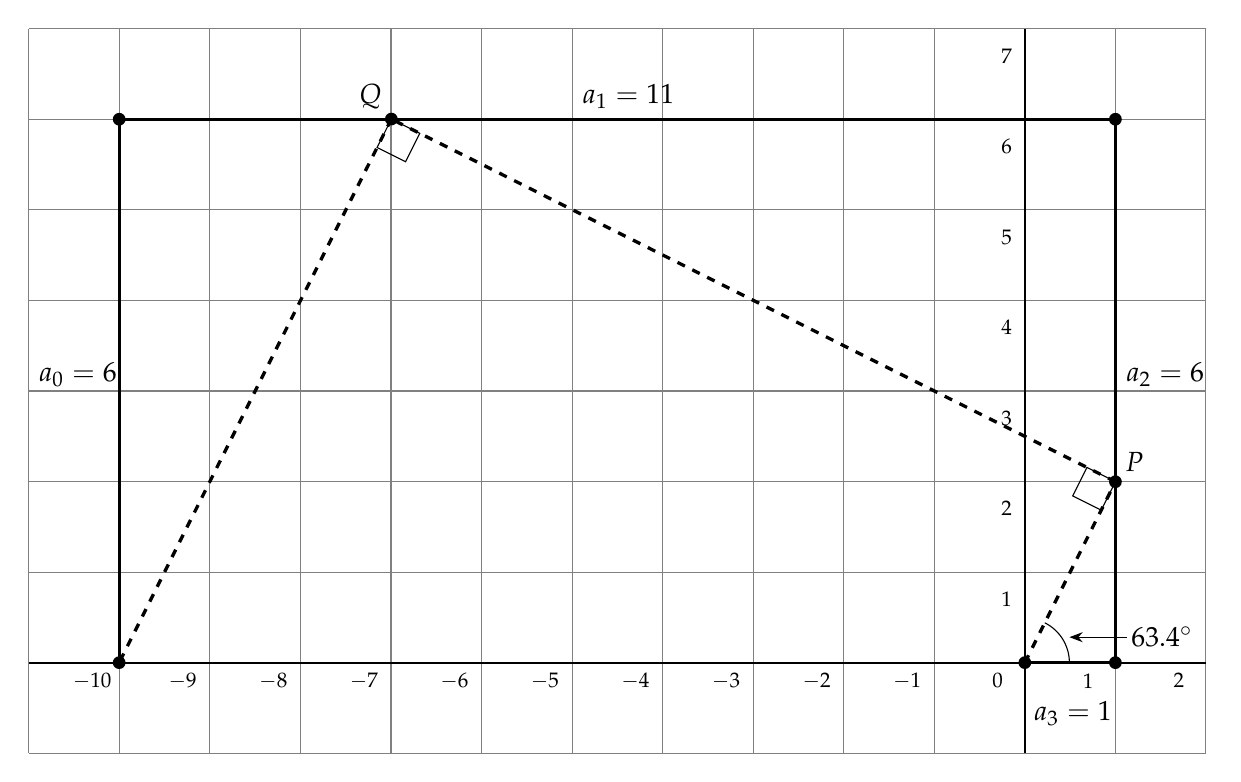
\begin{tikzpicture}[scale=1.15]
% Draw help lines and axes
\draw[step=10mm,white!50!black] (-11,-1) grid (2,7);
\draw[thick] (-11,0) -- (2,0);
\draw[thick] (0,-1) -- (0,7);
\foreach \x in {-10,...,2}
  \node at (\x-.3,-.2) {\sm{\x}};
\foreach \y in {1,...,7}
  \node at (-.2,\y-.3) {\sm{\y}};

% Draw first path
\coordinate (A) at (0,0);
\coordinate (B) at (1,0);
\coordinate (C) at (1,6);
\coordinate (D) at (-10,6);
\coordinate (E) at (-10,0);
\foreach \x in {A,B,C,D,E}
  \fill (\x) circle(2pt);
\draw[very thick] (A) --
  node[below,xshift=1pt,yshift=-10pt] {$a_3=1$} (B);
\draw[very thick,name path=bc] (B) -- 
  node[right,yshift=6pt] {$a_2=6$} (C);
\draw[very thick,name path=cd] (C) --
  node[above,xshift=4pt] {$a_1=11$}(D);
\draw[very thick,name path=de] (D) --
  node[left,xshift=3pt,yshift=6pt] {$a_0=6$}(E);

% Draw first segment of second path
\path[name path=a2] (A) -- +(63.4:4);
\path [name intersections = {of = a2 and bc, by = {A2}}];
\fill (A2) circle(2pt) node[above right] {$P$};
\draw[very thick,dashed] (A) -- (A2);
\draw ($(A) + (14pt,0)$)
  arc [start angle=0, end angle = 63.4, radius=14pt];
\node[above right,xshift=35pt,yshift=2pt] at (A) {$63.4^\circ$};
\draw[->] ($(A)+(32pt,8pt)$) -- +(-18pt,0);
\draw[rotate=153.4] (A2) rectangle +(10pt,10pt);

% Draw second segment of second path
\path[name path=b2] (A2) -- +(153.4:10);
\path [name intersections = {of = b2 and cd, by = {B2}}];
\fill (B2) circle(2pt) node[above left] {$Q$};
\draw[very thick,dashed] (A2) -- (B2);
\draw[rotate=243.4] (B2) rectangle +(10pt,10pt);

% Draw third segment of second path%
\draw[very thick,dashed] (B2) -- (E);
\end{tikzpicture}
\end{center}
Let $p(x)=a_3x^3+a_2x^2+a_1x+a_0=x^3+6x^2+11x+6$. Compute $\tan 63.4^\circ=2$, the tangent of the angle at the start of the first path. Then:
\[
p(-\tan 63.4^\circ)=(-2)^3+6(-2)^2+11(-2)+6=0\,.
\]
Congratulations! You have found a root of the cubic polynomial $x^3+6x^2+11x+6$.

\newpage

\section{Introduction}
This example demonstrates a method discovered by Eduard Lill in 1867 for graphically finding the real roots of any polynomial \cite{bradford, hull-beloch, riaz}. We limit the presentation to cubic polynomials.

Clearly, this is not an algebraic method of computing roots of cubic equations; in the example, we are essentially verifying that $-2$ is a root. Lill's method has seen renewed interest because it can be implemented using origami \cite{hull-beloch}.

In Sections~\ref{s.multiple}--\ref{s.noroots} we continue the initial example to find additional roots of the polynomial and to show that if an angle $\alpha$ is chosen such that $-\tan\alpha$ is \emph{not} a root, then the construction doesn't work.

Section~\ref{s.method} presents the full specification of Lill's method. Some of the description may be difficult to understand, but will be clarified when demonstrated by additional examples in Sections~\ref{s.negative}, \ref{s.zero}, \ref{s.noninteger}. Since Lill's method can find a real root of any cubic polynomial, it can be used to trisect an angle. Since it can find $\sqrt[3]{2}$ as a root of $x^3-2$, it can double a cube as shown in Section~\ref{s.cube}.

Section~\ref{s.proof} gives a proof that Lill's method can find the real roots of any cubic polynomial. The proof for arbitrary polynomials follows the same structure.

Section~\ref{s.beloch-fold} investigates the connection between Lill's method and origami and Section~\ref{s.beloch-square} presents Beloch's definition of origami Axiom~6 as a Beloch square.

\newpage

\section{Multiple roots}\label{s.multiple}

Let us continue the example above. The polynomial $p(x)=a_3x^3+6x^2+11x+6$ has three roots $-1,-2,-3$. Computing the arc tangent of the negation of the roots gives:
\[
\alpha=-\tan^{-1} -1 = 45^\circ,\quad \beta=-\tan^{-1}-2 = 63.4^\circ,\quad \gamma=-\tan^{-1} -3= 71.6^\circ\,.
\]
In the diagram below we see that for each of the three angles, the second path intersects the end of the first path.
\begin{center}
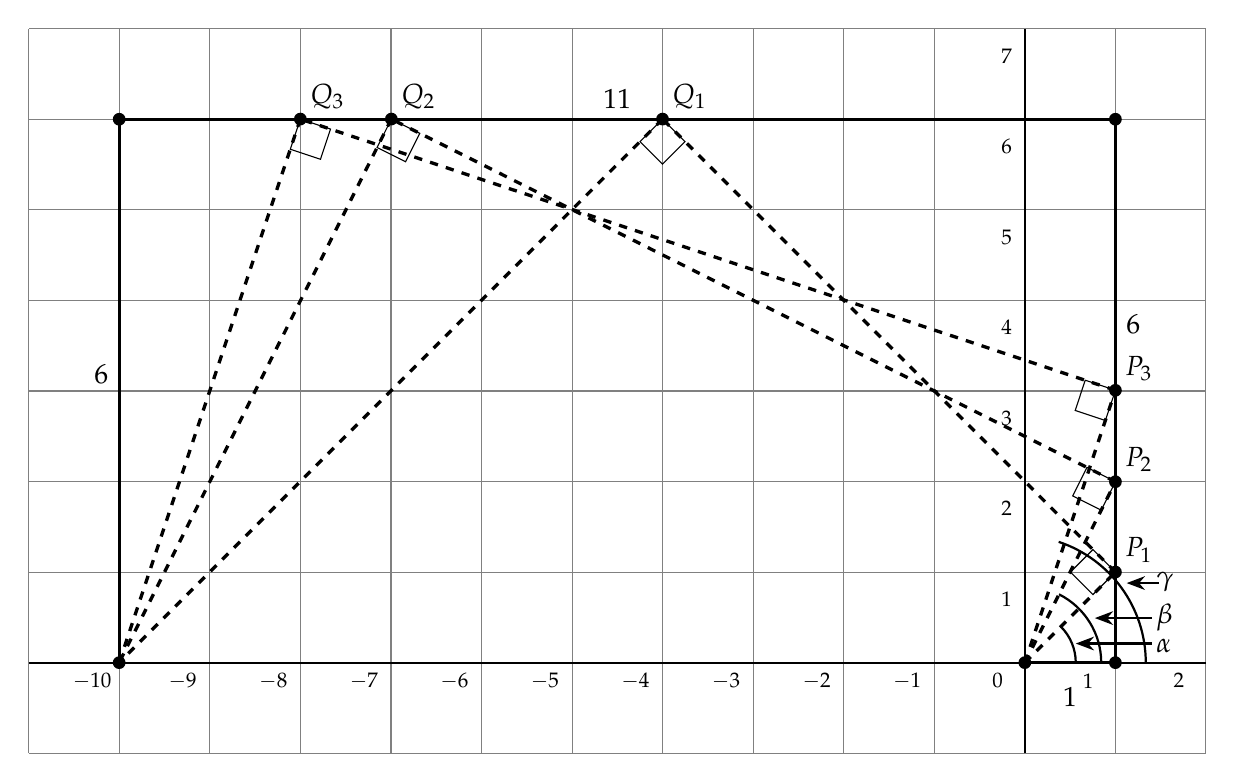
\begin{tikzpicture}[scale=1.15]
% Draw help lines and axes
\draw[step=10mm,white!50!black] (-11,-1) grid (2,7);
\draw[thick] (-11,0) -- (2,0);
\draw[thick] (0,-1) -- (0,7);
\foreach \x in {-10,...,2}
  \node at (\x-.3,-.2) {\sm{\x}};
\foreach \y in {1,...,7}
  \node at (-.2,\y-.3) {\sm{\y}};
\coordinate (A) at (0,0);
\coordinate (B) at (1,0);
\coordinate (C) at (1,6);
\coordinate (D) at (-10,6);
\coordinate (E) at (-10,0);
\foreach \x in {A,B,C,D,E}
  \fill (\x) circle(2pt);
\draw[very thick] (A) --
  node[below,yshift=-5pt] {$1$} (B);
\draw[very thick,name path=bc] (B) -- 
  node[right,yshift=24pt] {$6$} (C);
\draw[very thick,name path=cd] (C) --
  node[above] {$11$}(D);
\path[name path=de] (D) -- ($(E)+(0,-.8)$);
\draw[very thick] (D) --
  node[left,yshift=6pt] {$6$} (E);


% Draw first segment of first second path
\path[name path=a1] (A) -- +(45:3);
\path [name intersections = {of = a1 and bc, by = {A1}}];
\fill (A1) circle(2pt) node[above right] {$P_1$};
\draw[very thick,dashed] (A) -- (A1);
\draw[thick] ($(A) + (16pt,0)$)
  arc [start angle=0, end angle = 45, radius=16pt];
\node[above right,xshift=44pt,yshift=0pt] at (A) {$\alpha$};
\draw[rotate=135] (A1) rectangle +(10pt,10pt);
\draw[Stealth-,thick] ($(A) + (16pt,6pt)$) -- +(24pt,0);

% Draw second segment of first second path
\path[name path=b1] (A1) -- +(135:8);
\path [name intersections = {of = b1 and cd, by = {B1}}];
\fill (B1) circle(2pt) node[above right] {$Q_1$};
\draw[very thick,dashed] (A1) -- (B1);
\draw[rotate=225] (B1) rectangle +(10pt,10pt);

% Draw third segment of first second path
\draw[very thick,dashed] (B1) -- (E);

% Draw first segment of second second path
\path[name path=a2] (A) -- +(63.4:4);
\path [name intersections = {of = a2 and bc, by = {A2}}];
\fill (A2) circle(2pt) node[above right] {$P_2$};
\draw[very thick,dashed] (A) -- (A2);
\draw[thick] ($(A) + (24pt,0)$)
  arc [start angle=0, end angle = 63.4, radius=24pt];
\node[above right,xshift=44pt,yshift=8pt] at (A) {$\beta$};
\draw[rotate=153.4] (A2) rectangle +(10pt,10pt);
\draw[<-,thick] ($(A) + (22pt,14pt)$) -- +(18pt,0);

% Draw second segment of second second path%
\path[name path=b2] (A2) -- +(153.4:10);
\path [name intersections = {of = b2 and cd, by = {B2}}];
\fill (B2) circle(2pt) node[above right] {$Q_2$};
\draw[very thick,dashed] (A2) -- (B2);
\draw[rotate=243.4] (B2) rectangle +(10pt,10pt);

% Draw third segment of second second path%
\draw[very thick,dashed] (B2) -- (E);

% Draw first segment of second second path%
\path[name path=a3] (A) -- +(71.6:4);
\path [name intersections = {of = a3 and bc, by = {A3}}];
\fill (A3) circle(2pt) node[above right] {$P_3$};
\draw[very thick,dashed] (A) -- (A3);
\draw[thick] ($(A) + (38pt,0)$)
  arc [start angle=0, end angle = 71.6, radius=40pt];
\node[above right,xshift=44pt,yshift=22pt] at (A) {$\gamma$};
\draw[rotate=161.6] (A3) rectangle +(10pt,10pt);
\draw[<-,thick] ($(A) + (32pt,25pt)$) -- +(10pt,0);

% Draw second segment of second second path%
\path[name path=b3] (A3) -- +(161.6:10);
\path [name intersections = {of = b3 and cd, by = {B3}}];
\fill (B3) circle(2pt) node[above right] {$Q_3$};
\draw[very thick,dashed] (A3) -- (B3);
\draw[rotate=251.6] (B3) rectangle +(10pt,10pt);

% Draw third segment of second second path%
\draw[very thick,dashed] (B3) -- (E);
\end{tikzpicture}
\end{center}

\newpage

\section{Paths that do not lead to roots}\label{s.noroots}

Perhaps the second path intersects the end of the first path for \emph{any} initial angle, for example, $56.3^\circ$. In the following diagram, the second path intersects the extension of the line segment for the coefficient $a_0$, but not at $(-10,0)$, the end of the first path. We conclude that $-\tan 56.3=-1.5$ is \emph{not} a root of the equation.
\begin{center}
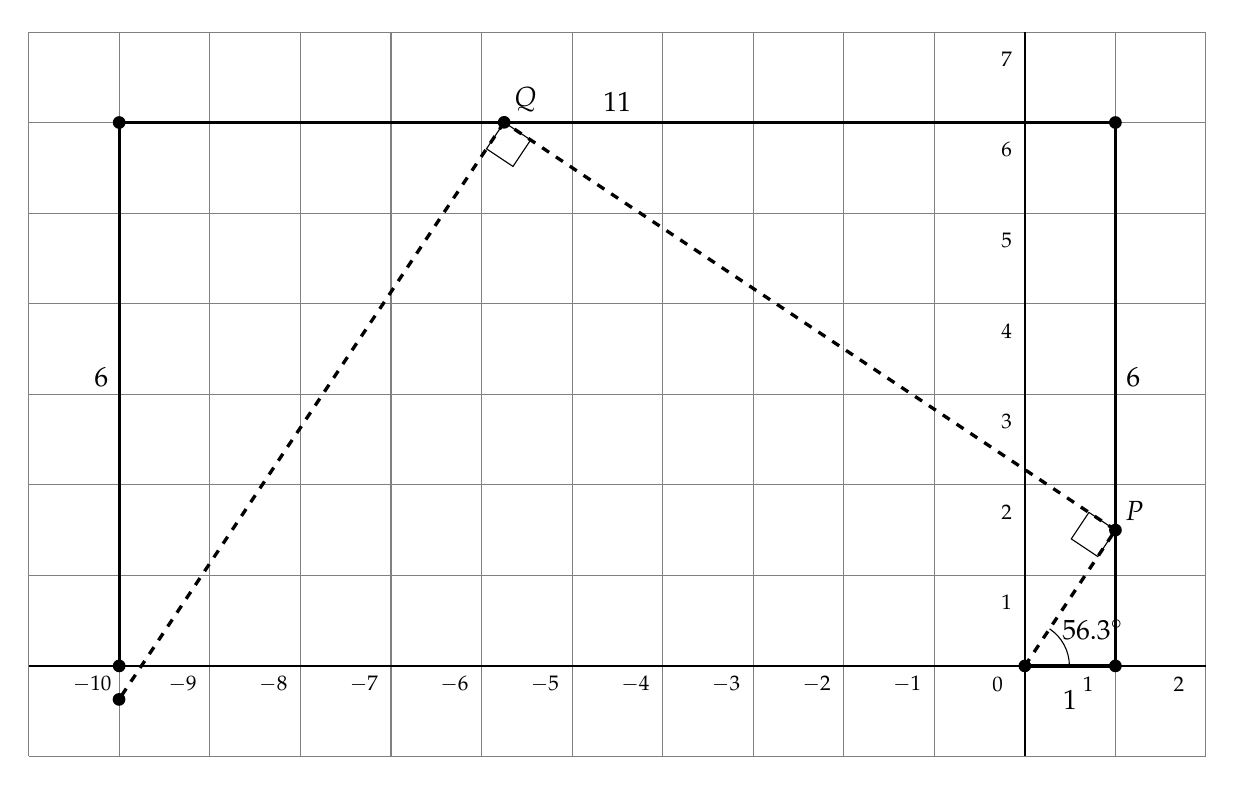
\begin{tikzpicture}[scale=1.15]
% Draw help lines and axes
\draw[step=10mm,white!50!black] (-11,-1) grid (2,7);
\draw[thick] (-11,0) -- (2,0);
\draw[thick] (0,-1) -- (0,7);
\foreach \x in {-10,...,2}
  \node at (\x-.3,-.2) {\sm{\x}};
\foreach \y in {1,...,7}
  \node at (-.2,\y-.3) {\sm{\y}};

% Draw first path
\coordinate (A) at (0,0);
\coordinate (B) at (1,0);
\coordinate (C) at (1,6);
\coordinate (D) at (-10,6);
\coordinate (E) at (-10,0);
\foreach \x in {A,B,C,D,E}
  \fill (\x) circle(2pt);
\draw[very thick] (A) --
  node[below,yshift=-5pt] {$1$} (B);
\draw[very thick,name path=bc] (B) -- 
  node[right,yshift=6pt] {$6$} (C);
\draw[very thick,name path=cd] (C) --
  node[above] {$11$}(D);
\draw[very thick] (D) --
  node[left,yshift=6pt] {$6$}(E);
\path[name path=de] (-10,-1) -- (-10,7);

% Draw first segment of second path
\path[name path=a2] (A) -- +(56.3:3);
\path [name intersections = {of = a2 and bc, by = {A2}}];
\fill (A2) circle(2pt) node[above right] {$P$};
\draw[very thick,dashed] (A) -- (A2);
\draw ($(A) + (14pt,0)$)
  arc [start angle=0, end angle = 56.3, radius=14pt];
\node[above right,xshift=10pt,yshift=6pt] at (A) {$56.3^\circ$};
\draw[rotate=146.3] (A2) rectangle +(10pt,10pt);

% Draw second segment of second path
\path[name path=b2] (A2) -- +(146.3:10);
\path [name intersections = {of = b2 and cd, by = {B2}}];
\fill (B2) circle(2pt) node[above right] {$Q$};
\draw[very thick,dashed] (A2) -- (B2);
\draw[rotate=236.3] (B2) rectangle +(10pt,10pt);

% Draw third segment of second path
\path[name path=c2] (B2) -- +(236.3:8.5);
\path [name intersections = {of = c2 and de, by = {C2}}];
\fill (C2) circle(2pt);
\draw[very thick,dashed] (B2) -- (C2);
\end{tikzpicture}
\end{center}

\newpage

\section{Specification of Lill's method}\label{s.method}

This section gives the complete specification of Lill's method for finding real roots of cubic polynomials. Examining the examples below will help understand the details.
\begin{itemize}
\item Start with an arbitrary cubic polynomial: $p(x)=a_3x^3+a_2x^2+a_1x+a_0$.
\item Construct the first path as follows:
\begin{itemize}
\item For each coefficient $a_3,a_2,a_1,a_0$ (in that order) draw a line segment starting at the origin $O=(0,0)$ in the positive direction of the $x$-axis. Turn $90^\circ$ counterclockwise between each segment.
\end{itemize}
\item Construct the second path as follows:
\begin{itemize}
\item We use $a_i$ to denote the side of length $a_i$.
\item Construct a line from $O$ at an angle of $\theta$ with the positive $x$-axis that intersects $a_2$ at point $P$.
\item Turn $\pm 90^\circ$ and construct a line from $P$ that intersects $a_1$ at $Q$.
\item Turn $\pm 90^\circ$ and construct a line from $Q$ that intersects $a_0$ at $R$.
\item If $R$ is the end point of the first path, then $-\tan\theta$ is a root of $p(x)$.
\end{itemize}
\item Special cases:
\begin{itemize}
\item When drawing the line segments of the first path, if a coefficient is negative, draw the line segment \emph{backwards}.
\item When drawing the line segments of the first path, if a coefficient is zero, do not draw a line segment but continue with the next $\pm90^\circ$ turn.
\end{itemize}
\item Notes:
\begin{itemize}
\item "Intersects $a_i$" includes ``intersects with the line that contains $a_i$''.
\item When building the second path, choose to turn left or right by $90^\circ$ so that there is an intersection with the next segment of the first path.
\end{itemize}
\end{itemize}

\newpage

\section{Negative coefficients}\label{s.negative}

In \cite{moti-origami} I gave an example of the use of origami Axiom~6 which results in the polynomial $p(x)=x^3-3x^2-3x+1$ which has negative coefficients.

We start by drawing a segment of length $1$ to the right. Next we turn $90^\circ$ to face up, but the coefficient is negative, so we draw a segment of length $3$ \emph{down}. After turning $90^\circ$ to the left, the coefficient is again negative, so we draw a segment of length $3$ to the right. Finally, we turn down and draw a segment of length $1$.

We start the second path with a line angled $45^\circ$ with the $x$-axis. It intersects the \emph{extension} of the line segment for $a_2$ at $(1,1)$. Turning $-90^\circ$ (to the right), the line intersects the \emph{extension} of the line segment for $a_1$ at $(5,-3)$. Turning $-90^\circ$ again, the line intersects the end of the first path at $(4,-4)$.

Since $-\tan 45^\circ=-1$, a real root of the polynomial is $-1$:
\[
p(-1)=(-1)^3-3(-1)^2-3(-1)+6=-1-3+3+1=0\,.
\]
The loosely dashed lines in the Figure will be discussed  in Section~\ref{s.noninteger}.

\begin{center}
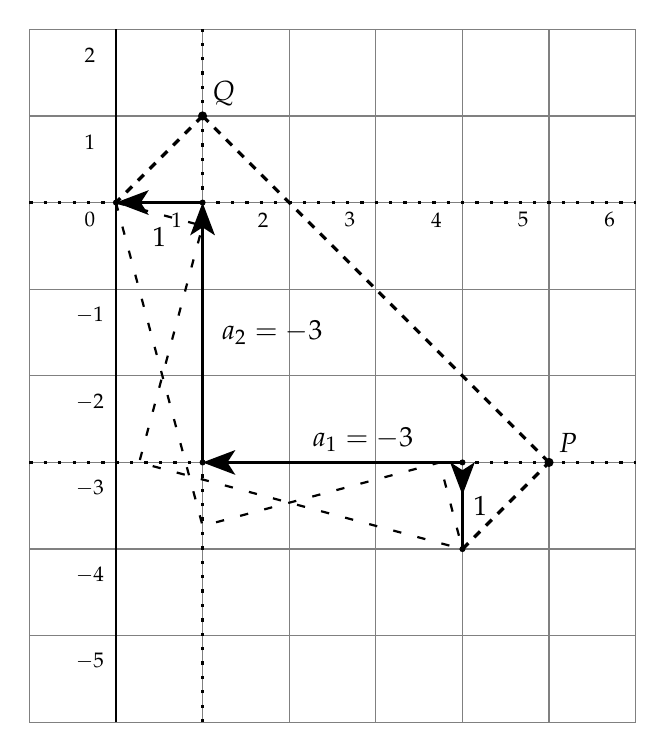
\begin{tikzpicture}[scale=1.1]
% Draw help lines and axes
\draw[step=10mm,white!50!black] (-1,-6) grid (6,2);
\draw (0,-6) -- (0,2);
\foreach \x in {0,...,6}
  \node at (\x-.3,-.2) {\sm{\x}};
\foreach \y in {-5,...,-1}
  \node at (-.3,\y-.3) {\sm{\y}};
\foreach \y in {1,...,2}
  \node at (-.3,\y-.3) {\sm{\y}};

% Draw first path
\coordinate (A) at (0,0);
\coordinate (B) at (1,0);
\coordinate (C) at (1,-3);
\coordinate (D) at (4,-3);
\coordinate (E) at (4,-4);
\foreach \x in {A,B,C,D,E}
  \fill (\x) circle(1pt);
\draw[very thick,{Stealth[scale=1.4,inset=2pt]}-] (A) --
  node[below,yshift=-5pt] {$1$} (B);
\draw[very thick,{Stealth[scale=1.4,inset=2pt]}-,name path=bc] (B) -- 
  node[right,xshift=3pt] {$a_2=-3$} (C);
\draw[very thick,{Stealth[scale=1.4,inset=2pt]}-,name path=cd] (C) --
  node[above,xshift=11pt] {$a_1=-3$}(D);
\draw[very thick,{Stealth[scale=1.4,inset=2pt,reversed]}-,name path=de] (D) --
  node[right] {$1$}(E);

% Draw extensions of first path
\draw[very thick,loosely dotted,name path=a] (-1,0) -- (6,0);
\draw[very thick,loosely dotted,name path=b] (1,-6) -- (1,2);
\draw[very thick,loosely dotted,name path=c] (-1,-3) -- (6,-3);

% Draw first second path
\path[name path=a1] (A) -- +(-75:5);
\path [name intersections = {of = a1 and b, by = {B1}}];
\path[name path=b1] (B1) -- +(15:5);
\path [name intersections = {of = b1 and c, by = {C1}}];
\draw[thick,loosely dashed] (A) -- (B1) -- (C1) -- (E);

% Draw second second path
\draw[very thick,dashed] (4,-4) -- (5,-3) coordinate (A2);
\fill (5,-3) circle (1.5pt) node[above right] {$P$};
\draw[very thick,dashed] (5,-3) -- (1,1) coordinate (B2);
\fill (1,1) circle (1.5pt) node[above right] {$Q$};
\draw[very thick,dashed] (1,1) -- (0,0);

% Draw third second path
\path[name path=a3] (A) -- +(-15:5);
\path [name intersections = {of = a3 and b, by = {B3}}];
\path[name path=b3] (B3) -- +(-105:5);
\path [name intersections = {of = b3 and c, by = {C3}}];
\draw[thick,loosely dashed] (A) -- (B3) -- (C3) -- (E);
\end{tikzpicture}
\end{center}

\newpage

\section{Zero coefficients}\label{s.zero}

$a_2$, the coefficient of the $x^2$ term in the polynomial $x^3-7x-6=0$, is zero. For a zero coefficient, we ``draw'' a line segment of length $0$, that is, we do not draw a line, but we still make the $\pm 90^\circ$ turn before ``drawing'' it, as indicated by the arrow pointed up at point $(1,0)$ in the diagram. Next make an additional turn and draw a line of length $-7$, that is, of length $7$ backwards, to point $(8,0)$. Finally, turn again and draw a line of length $-6$ to point $(8,6)$.

There are three second paths that intersect the end of the first path. They start with angles of:
\[
\alpha=45^\circ,\; \beta=63.4^\circ,\; \gamma=-71.6^\circ\,.
\]
We conclude that there are three real roots:
\[
-\tan 45^\circ=-1,\; -\tan 63.4^\circ =-2,\; -\tan -71.6^\circ=3\,.
\]
Check:
\[
(x+1)(x+2)(x-3)=(x^2+3x+2)(x-3) =x^3-7x-6\,.
\]

\begin{center}
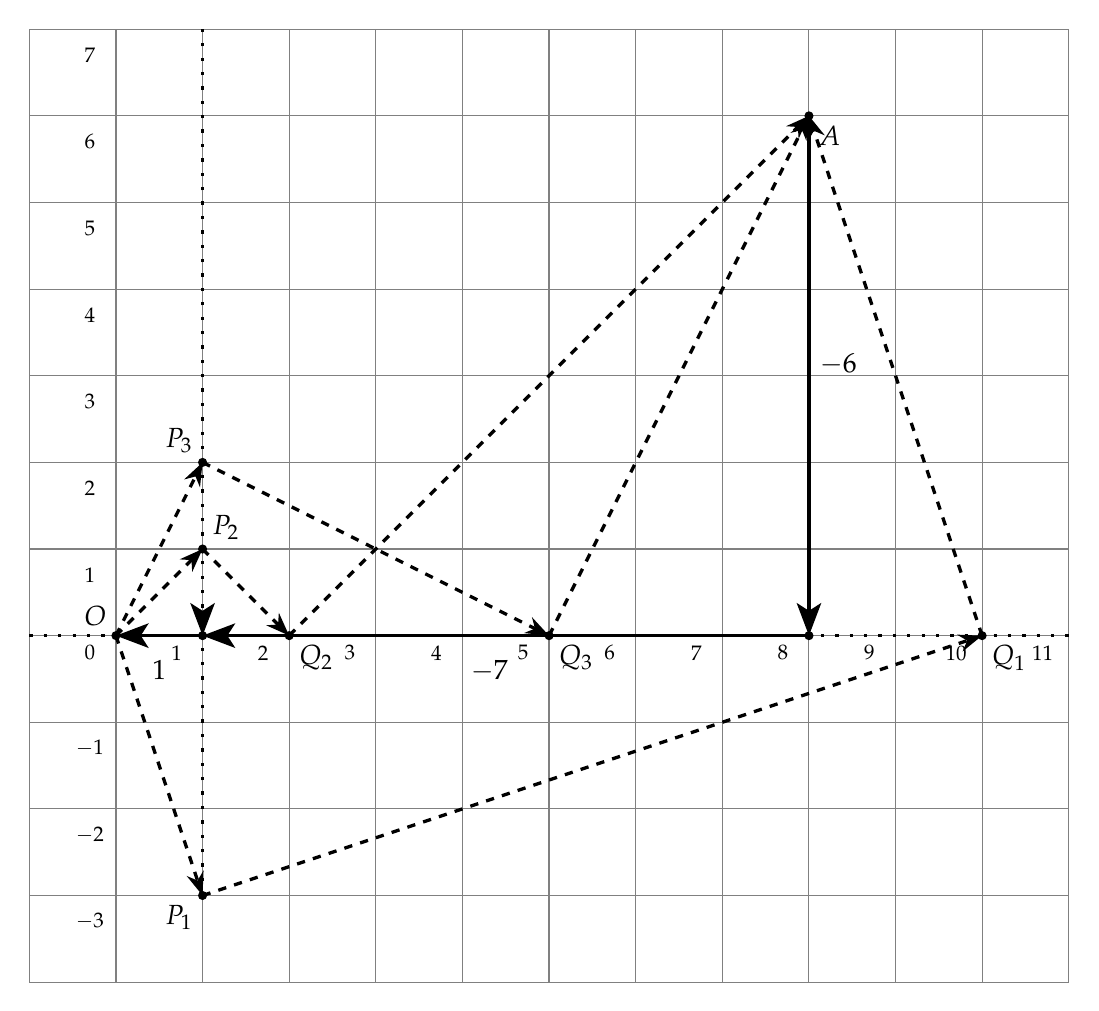
\begin{tikzpicture}[scale=1.1]
% Draw help lines and axes
\draw[step=10mm,white!50!black] (-1,-4) grid (11,7);
\foreach \x in {0,...,11}
  \node at (\x-.3,-.2) {\sm{\x}};
\foreach \y in {-3,...,-1}
  \node at (-.3,\y-.3) {\sm{\y}};
\foreach \y in {1,...,7}
  \node at (-.3,\y-.3) {\sm{\y}};

% Draw first path
\coordinate (A) at (0,0) node[above left] {$O$};
\coordinate (B) at (1,0);
\coordinate (C) at (8,0);
\coordinate (D) at (8,6);
\node[below right] at (D) {$A$};
\foreach \x in {A,B,C,D}
  \fill (\x) circle(1.5pt); 
\draw[very thick,{Stealth[scale=1.4,inset=2pt]}-] (A) --
  node[below,yshift=-5pt] {$1$} (B);
\draw[{Stealth[scale=1.4,inset=2pt]}-,very thick] (B) --
  ($(B)+(0,.1)$);
\draw[very thick,{Stealth[scale=1.4,inset=2pt]}-,name path=bc] (B) -- 
  node[below,xshift=-6pt,yshift=-5pt] {$-7$} (C);
\draw[very thick,{Stealth[scale=1.4,inset=2pt]}-,name path=cd] (C) --
  node[right,yshift=4pt] {$-6$}(D);

% Draw extensions of first path
\draw[very thick,loosely dotted] (1,-3) -- (1,7);
\draw[very thick,loosely dotted] (-1,0) -- (11,0);

% Draw first second path
\draw[very thick,dashed,->] (0,0) -- (1,-3);
\fill (1,-3) circle (1.5pt) node[below left] {$P_1$};
\draw[very thick,dashed,->] (1,-3) coordinate (A1) -- (10,0);
\fill (10,0) circle (1.5pt) node[below right] {$Q_1$};
\draw[very thick,dashed,->] (10,0) coordinate (B1) -- (D);

% Draw second second path
\draw[very thick,dashed,->] (0,0) -- (1,1) coordinate (A2);
\fill (A2) circle (1.5pt) node[above right] at (A2) {$P_2$};
\draw[very thick,dashed,->] (A2) -- (2,0) coordinate (B2);
\fill (B2) circle (1.5pt) node[below right] at (B2) {$Q_2$};
\draw[very thick,dashed,->] (B2) -- (D);

% Draw third second path
\draw[very thick,dashed,->] (0,0) -- (1,2) coordinate (A3);
\fill (A3) circle (1.5pt) node[above left] {$P_3$};
\draw[very thick,dashed,->] (A3) -- (5,0) coordinate (B3);
\fill (B3) circle (1.5pt) node[below right] at (B3) {$Q_3$};
\draw[very thick,dashed,->] (B3) -- (D);
\end{tikzpicture}
\end{center}

\newpage

\section{Non-integer roots}\label{s.noninteger}

Consider the polynomial $p(x)=x^3-2x+1$. The first path goes from $(0,0)$ to $(1,0)$ and then turns up. The coefficient of $x^2$ is zero so no segment is drawn and the path turns left. The next segment is of length $-2$ so it goes backwards from $(1,0)$ to $(3,0)$. Finally, the path turns down and a line of length $1$ is drawn from $(3,0)$ to $(3,-1)$.


It is easy to see that $1$ is a root of $p(x)$. Since $-\tan^{-1} -45^\circ=-1$, there is a path $\overline{OP_1Q_1A}$.

 If we divide $p(x)$ by $x-1$, we obtain the quadratic polynomial $x^2+x-1$ whose roots are:
\[
\disfrac{-1\pm\sqrt{5}}{2} \approx 0.62,\; -1.62\,.
\]
Therefore, there are two additional second paths: one starting with an angle of $-31.8^\circ$ since $-\tan^{-1} 0.62=-31.8^\circ$, and one starting with $58.3^\circ$ since $-\tan^{-1}1.62=58.3^\circ$.

Similarly, the polynomial in Section~\ref{s.negative} has roots $ 2\pm\sqrt{3}\approx 3.73, 0.27$. The corresponding angles are $-75^\circ$ and $-15^\circ$, because $(-\tan -75^\circ)\approx 3.73$ and $(-\tan -15^\circ)\approx 0.27$.
\begin{center}
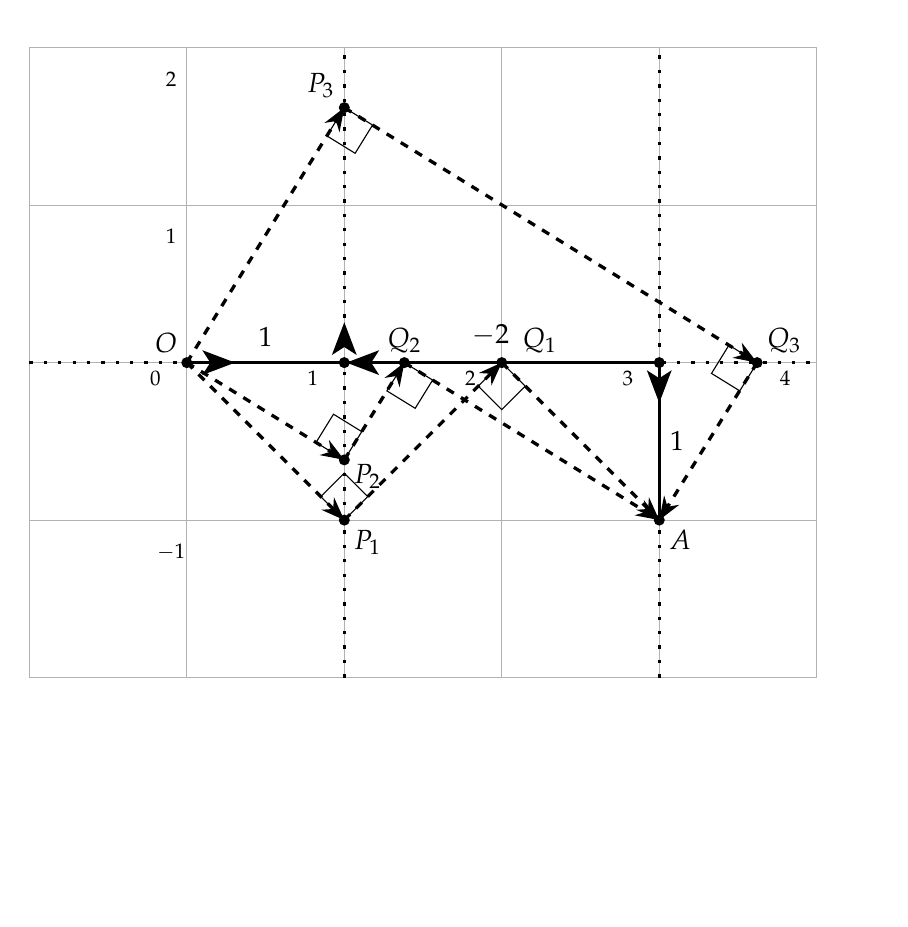
\begin{tikzpicture}[scale=2]
% Draw help lines and axes
\draw[step=10mm,white!70!black,] (-1,-2) grid (4,2);
\foreach \x in {0,...,4}
  \node at (\x-.2,-.1) {\sm{\x}};
\foreach \y in {-1}
  \node at (-.1,\y-.2) {\sm{\y}};
\foreach \y in {1,2}
  \node at (-.1,\y-.2) {\sm{\y}};

% Draw first path
\coordinate (A) at (0,0);
\node[above left] at (A) {$O$};
\coordinate (B) at (1,0);
\coordinate (C) at (3,0);
\coordinate (D) at (3,-1);
\node[below right] at (D) {$A$};
\foreach \x in {A,B,C,D}
  \fill (\x) circle(1pt); 
\draw[very thick] (A) -- node[above,yshift=2pt] {$1$} (B);
\draw[{Stealth[scale=1.4,inset=2pt,reversed]}-,very thick] ($(A)+(.1,0)$) --
  ($(A)+(.15,0)$);
\draw[{Stealth[scale=1.4,inset=2pt,reversed]}-,very thick] ($(B)+(0,.05)$) --
  ($(B)+(0,.1)$);
\draw[very thick,name path=bc] (B) -- 
  node[above,xshift=-4pt,yshift=2pt] {$-2$} (C);
\draw[{Stealth[scale=1.4,inset=2pt,reversed]}-,very thick] ($(B)+(.22,0)$) --
  ($(B)+(.17,0)$);
\draw[very thick,name path=cd] (C) --
  node[right] {$1$}(D);
\draw[{Stealth[scale=1.4,inset=2pt,reversed]}-,very thick] ($(C)+(0,-.05)$) --
 ($(C)+(0,-.1)$);

% Draw extensions of first path
\draw[very thick,loosely dotted,name path=b] (1,-2) -- (1,2);
\draw[very thick,loosely dotted,name path=c] (-1,0) -- (4,0);
\draw[very thick,loosely dotted,name path=d] (3,-2) -- (3,2);

% Draw first second path
\coordinate (A1) at (1,-1);
\draw[very thick,dashed,->] (0,0) -- (A1);
\fill (A1) circle (1pt) node[below right] {$P_1$};
\coordinate (B1) at (2,0);
\draw[very thick,dashed,->] (A1) -- (B1);
\fill (B1) circle (1pt) node[above right,xshift=4pt] {$Q_1$};
\draw[very thick,dashed,->] (B1) -- (D);
\draw[rotate=45] (A1) rectangle +(6pt,6pt);
\draw[rotate=-135] (B1) rectangle +(6pt,6pt);

% Draw second second path
\path[name path=a2] (0,0) -- +(-31.7:4);
\path [name intersections = {of = a2 and b, by = {A2}}];
\draw[very thick,dashed,->] (0,0) -- (A2);
\fill (A2) circle (1pt) node[below right,yshift=2pt] {$P_2$};
\path[name path=b2] (A2) -- +(58.3:2.5);
\path [name intersections = {of = b2 and c, by = {B2}}];
\draw[very thick,dashed,->] (A2) -- (B2);
\fill (B2) circle (1pt) node[above] {$Q_2$};
\draw[very thick,dashed,->] (B2) -- (D);
\draw[rotate=58.3]   (A2) rectangle +(6pt,6pt);
\draw[rotate=-121.7] (B2) rectangle +(6pt,6pt);

% Draw third second path
\path[name path=a3] (0,0) -- +(58.3:2.5);
\path [name intersections = {of = a3 and b, by = {A3}}];
\draw[very thick,dashed,->] (0,0) -- (A3);
\fill (A3) circle (1pt) node[above left] {$P_3$};
\path[name path=b3] (A3) -- +(-31.7:4);
\path [name intersections = {of = b3 and c, by = {B3}}];
\draw[very thick,dashed,->] (A3) -- (B3);
\fill (B3) circle (1pt) node[above right] {$Q_3$};
\path[name path=c3] (B3) -- +(-121.7:4);
\draw[very thick,dashed,->] (B3) -- (D);
\draw[rotate=-121.7]   (A3) rectangle +(6pt,6pt);
\draw[rotate=-211.7]   (B3) rectangle +(6pt,6pt);
\end{tikzpicture}
\end{center}

\newpage

\section{The cube root of two}\label{s.cube}

To double a cube we need to compute $\sqrt[3]{2}\approx 1.26$ which is a root of the cubic polynomial $x^3-2$. In the construction of the first path, we turn twice without drawing any line segments, because $a_2$ and $a_1$ are both zero. The first segment of the second path is drawn at an angle of $-51.6^\circ$ and $(-\tan -51.6^\circ)\approx 1.26\approx \sqrt[3]{2}$.

\begin{center}
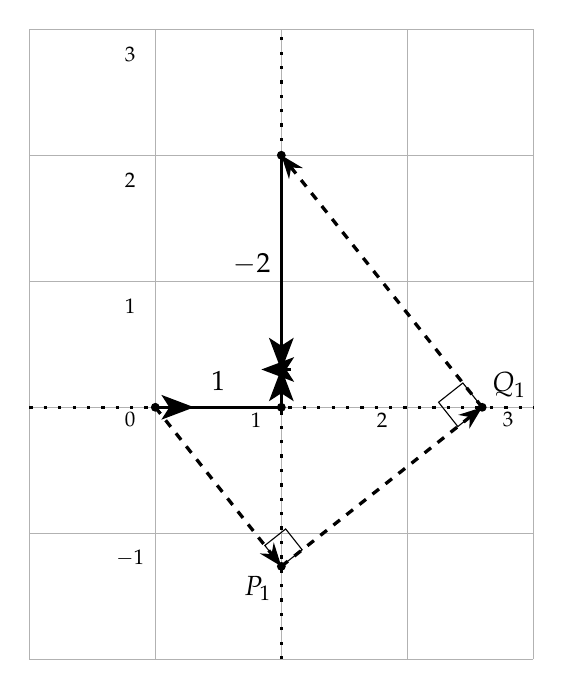
\begin{tikzpicture}[scale=1.6]
% Draw help lines and axes
\draw[step=10mm,white!70!black,] (-1,-2) grid (3,3);
\foreach \x in {0,...,3}
  \node at (\x-.2,-.1) {\sm{\x}};
\foreach \y in {-1}
  \node at (-.2,\y-.2) {\sm{\y}};
\foreach \y in {1,2,3}
  \node at (-.2,\y-.2) {\sm{\y}};

% Draw first path
\coordinate (A) at (0,0);
\coordinate (B) at (1,0);
\coordinate (C) at (1,2);
\foreach \x in {A,B,C}
  \fill (\x) circle(1pt); 
\draw[very thick] (A) -- node[above,yshift=2pt] {$1$} (B);

\draw[{Stealth[scale=1.4,inset=2pt,reversed]}-,very thick] ($(A)+(.05,0)$) --
  ($(A)+(.1,0)$);
\draw[{Stealth[scale=1.4,inset=2pt,reversed]}-,very thick] ($(B)+(0,.05)$) --
  ($(B)+(0,.1)$);
\draw[{Stealth[scale=1.4,inset=2pt,reversed]}-,very thick] ($(B)+(.1,.3)$) --
  ($(B)+(.08,.3)$);
\draw[{Stealth[scale=1.4,inset=2pt,reversed]}-,very thick] ($(B)+(0,.55)$) --
  ($(B)+(0,.5)$);

\draw[very thick] (B) -- 
  node[left,yshift=6pt] {$-2$} (C);

% Draw extensions of first path
\draw[very thick,loosely dotted,name path=a] (-1,0) -- (3,0);
\draw[very thick,loosely dotted,name path=b] (1,-2) -- (1,3);

% Draw first segment of second path
\path[name path=a1] (0,0) -- +(-51.6:2);
\path [name intersections = {of = a1 and b, by = {A1}}];
\draw[very thick,dashed,->] (A) -- (A1);
\fill (A1) circle (1pt) node[below left] {$P_1$};
\draw[rotate=38.4]   (A1) rectangle +(6pt,6pt);

% Draw second segment of second path
\path[name path=b1] (A1) -- +(38.4:2.5);
\path [name intersections = {of = b1 and a, by = {B1}}];
\draw[very thick,dashed,->] (A1) -- (B1);
\fill (B1) circle (1pt) node[above right] {$Q_1$};
\draw[rotate=128.4] (B1) rectangle +(7pt,7pt);

% Draw third segement of second path
\draw[very thick,dashed,->] (B1) -- (C);
\end{tikzpicture}
\end{center}
\begin{comment}
Once we have a real root of two, we can compute the two complex roots as follows. Since $\sqrt[3]{2}=\sqrt[3]{2\cdot 1}=\sqrt[3]{2}\cdot\sqrt[3]{1}$, it is sufficient to find the cube roots of one, that is, the roots of the polynomial $x^3-1$. One root is $1$ and dividing by $x-1$ gives a quadratic equation:
\[
x^3-1=(x-1)(x^2+x+1)\,.
\]
Now use the formula for finding the roots of a quadratic polynomial:
\[
r=\disfrac{-1\pm\sqrt{b^2-4ac}}{2}=\disfrac{-1\pm\sqrt{1-4}}{2}=\disfrac{-1\pm i\sqrt{3}}{2}\,.
\]
Check that:
\[
\left(\sqrt[3]{2}\cdot \disfrac{-1\pm i\sqrt{3}}{2}\right)^3=2\,.
\]
\end{comment}

\newpage

\section{Proof of Lill's method}\label{s.proof}

We limit ourselves to monic cubic polynomials $p(x)=x^3+a_2x^2+a_1x+a_0$.\footnote{If the polynomial is not monic, divide it by $a_3$ and the resulting monic polynomial has the same roots.} In the diagram below, segments of the first path are labeled with coefficients and with $b_2,b_1,a_2-b_2,a_1-b_1$.

Since the sum of the angles of a triangle is $180^\circ$, in a right triangle if one acute angle is $\theta$, the other is $90^\circ-\theta$. Therefore, the angles above $P$ and the angle to the left of $Q$ are equal to $\theta$. We now derive a sequence of formulas for $\tan \theta$:
\begin{form}{1.5}
\tan \theta &=& \disfrac{b_2}{1}=b_2\\
%a_2-b_2&=&a_2-\tan\theta\\
\tan \theta &=& \disfrac{b_1}{a_2-b_2}=\disfrac{b_1}{a_2-\tan\theta}\\
b_1&=&\tan\theta (a_2-\tan\theta)\\
\tan \theta &=& \disfrac{a_0}{a_1-b_1}=\disfrac{a_0}{a_1-\tan\theta(a_2-\tan\theta)}\,.
\end{form}
Simplifying the last equation gives:
\begin{form}{1.2}
(\tan\theta)^3-a_2(\tan\theta)^2+a_1(\tan\theta)-a_0&=&0\\
-(\tan\theta)^3+a_2(\tan\theta)^2-a_1(\tan\theta)+a_0&=&0\\
(-\tan\theta)^3+a_2(-\tan\theta)^2+a_1(-\tan\theta)+a_0&=&0\,.
\end{form}
We conclude that $-\tan\theta$ is a real root of $x^3+a_2x^2+a_1x+a_0$.


\begin{center}
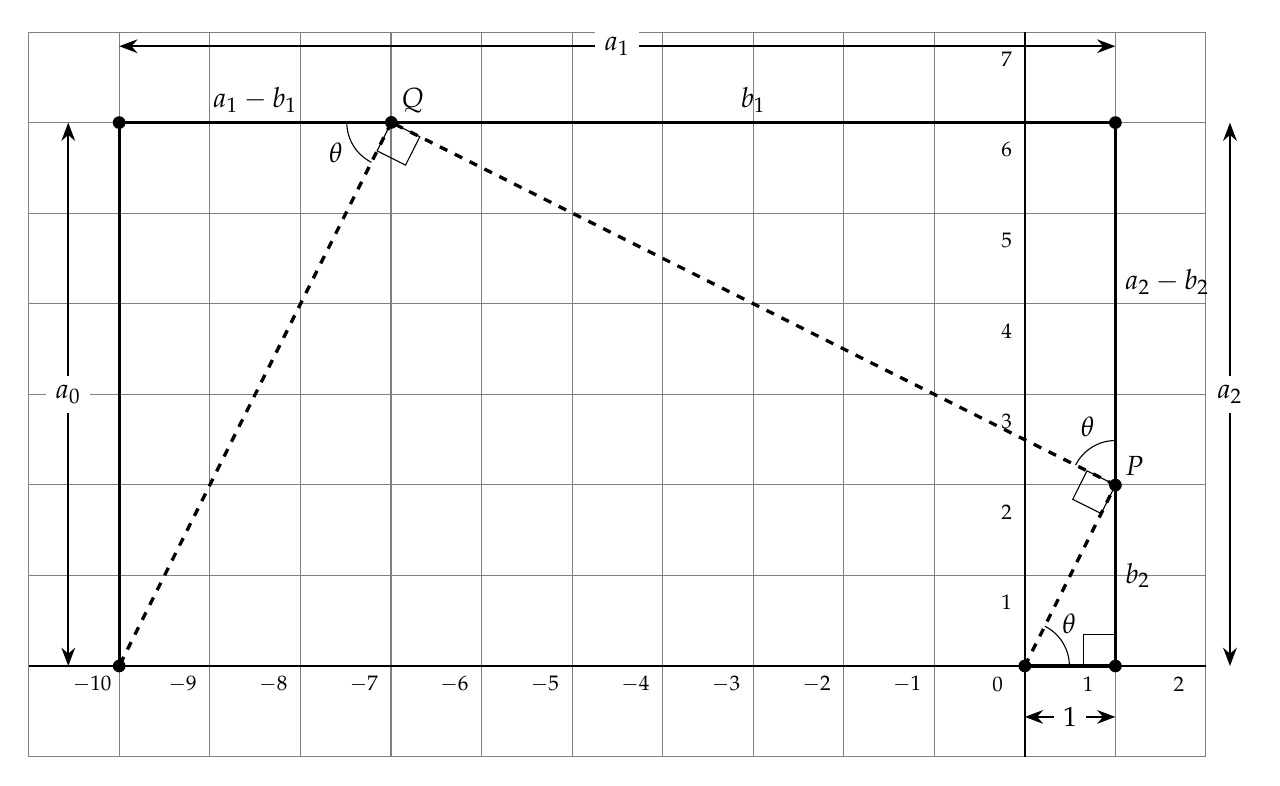
\begin{tikzpicture}[scale=1.15]
% Draw grid and axes
\draw[step=10mm,white!50!black] (-11,-1) grid (2,7);
\draw[thick] (-11,0) -- (2,0);
\draw[thick] (0,-1) -- (0,7);
\foreach \x in {-10,...,2}
  \node at (\x-.3,-.2) {\sm{\x}};
\foreach \y in {1,...,7}
  \node at (-.2,\y-.3) {\sm{\y}};
  
% Draw the points of the first path
\coordinate (A) at (0,0);
\coordinate (B) at (1,0);
\coordinate (C) at (1,6);
\coordinate (D) at (-10,6);
\coordinate (E) at (-10,0);
\foreach \x in {A,B,C,D,E}
  \fill (\x) circle(2pt);
\draw[rotate=90] (B) rectangle +(10pt,10pt);
  
% Draw A -- B and arrow
\draw[very thick] (A) --(B);
\draw[thick,<->] ($(A)+(0,-16pt)$) --
  node[fill=white] {$1$} ($(B)+(0,-16pt)$);

% Draw B -- C and arrow
\draw[very thick,name path=bc] (B) -- (C);
\draw[thick,<->] ($(B)+(36pt,0)$) --
  node[fill=white] {$a_2$} ($(C)+(36pt,0)$);

% Draw C -- D and arrow
\draw[very thick,name path=cd] (C) --(D);
\draw[thick,<->] ($(C)+(0,24pt)$) -- 
  node[fill=white] {$a_1$} ($(D)+(0,24pt)$);

% Draw D -- E and arrow
\draw[very thick,name path=de] (D) -- (E);
\draw[thick,<->] ($(D)+(-16pt,0)$) --
  node[fill=white] {$a_0$} ($(E)+(-16pt,0)$);

% Draw first angled segment of the second path and intersection A2 with BC
\path[name path=a2] (A) -- +(63.4:4);
\path [name intersections = {of = a2 and bc, by = {A2}}];
\fill (A2) circle(2pt) node[above right] {$P$};
\draw[very thick,dashed] (A) -- (A2);
\path (B) -- node[right] {$b_2$} (A2);
\path (A2) -- node[right,yshift=8pt] {$a_2-b_2$} (C);
\draw[rotate=153.4] (A2) rectangle +(10pt,10pt);

% Draw second segment of the second path and intersection B2 with CD
\path[name path=b2] (A2) -- +(153.4:10);
\path [name intersections = {of = b2 and cd, by = {B2}}];
\fill (B2) circle(2pt) node[above right] {$Q$};
\draw[very thick,dashed] (A2) -- (B2);
\draw[rotate=243.4] (B2) rectangle +(10pt,10pt);
\path (D) -- node[above] {$a_1-b_1$} (B2); 
\path (B2) -- node[above] {$b_1$} (C);

% Draw third segment of the second path to E
\draw[very thick,dashed] (B2)-- (E);

% Label A, A2, B2 with theta
\draw ($(A) + (14pt,0)$)
  arc [start angle=0, end angle = 63.4, radius=14pt];
\node[above right,xshift=10pt,yshift=8pt] at (A) {$\theta$};
\draw ($(A2) + (0,14pt)$)
  arc [start angle=90, end angle = 153.4, radius=14pt];
\node[above left,xshift=-4pt,yshift=14pt] at (A2) {$\theta$};
\draw ($(B2) + (-14pt,0)$)
  arc [start angle=180, end angle = 243.4, radius=14pt];
\node[below left,xshift=-14pt,yshift=-4pt] at (B2) {$\theta$};
\end{tikzpicture}
\end{center}

\newpage

\section{The Beloch fold}\label{s.beloch-fold}

Margharita P. Beloch discovered a remarkable connection between origami and Lill's method for solving cubic equations. She found that one application of the operation of origami Axiom~6 \cite[Section~8]{moti-origami} applied to the first path of Lill's method can obtain a real root of any cubic polynomial. The operation is often called the \emph{Beloch fold} in her honor.

Consider the polynomial $p(x)=x^3+6x^2+11x+6$ from Section~\ref{s.magic}. In the following diagram we have emphasized the second path and renamed some vertices. All we have to do to solve the equation is to locate the points $P',Q'$ on the line segments of lengths $a_2,a_1$, respectively. This looks like an easy application of the Beloch fold. Unfortunately, if you apply the axiom, the path does not solve the equation: $Q'$ is way off to the right, so the angle at $P'$ and $Q'$ are not right angles.
\begin{center}
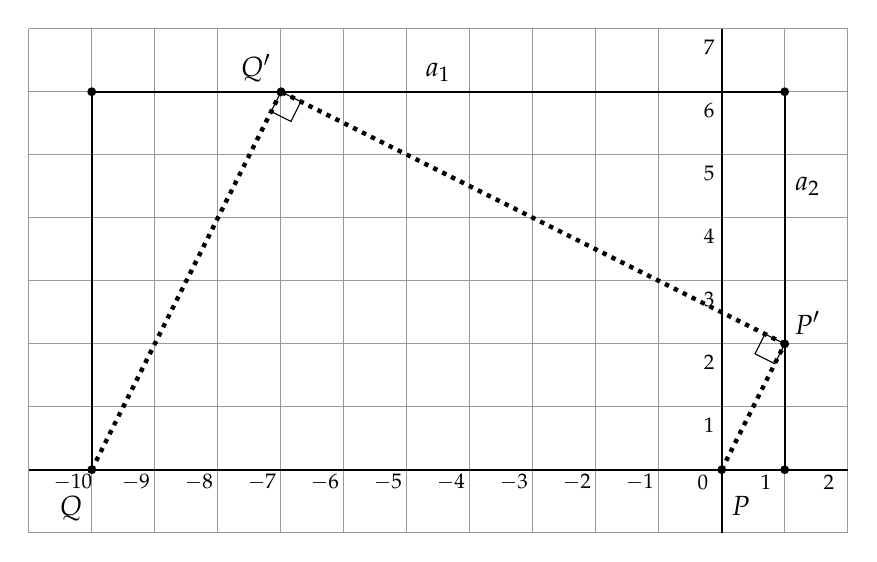
\begin{tikzpicture}[scale=.8]
% Draw help lines and axes
\draw[step=10mm,white!60!black] (-11,-1) grid (2,7);
\draw[thick] (-11,0) -- (2,0);
\draw[thick] (0,-1) -- (0,7);
\foreach \x in {-10,...,2}
  \node at (\x-.3,-.2) {\sm{\x}};
\foreach \y in {1,...,7}
  \node at (-.2,\y-.3) {\sm{\y}};
  
%Draw first path with five points
\coordinate (A) at (0,0);
\coordinate (B) at (1,0);
\coordinate (C) at (1,6);
\coordinate (D) at (-10,6);
\coordinate (E) at (-10,0);
\foreach \x in {A,B,C,D,E}
  \fill (\x) circle(2pt);
\node[below right,yshift=-6pt]  at (A) {$P$};
\node[below left,yshift=-6pt] at (E) {$Q$};

\draw[thick] (A) -- (B);
\draw[thick,name path=bc] (B) --
  node[right,near end] {$a_2$} (C);
\draw[thick,name path=cd] (C) -- 
  node[above] {$a_1$} (D);
\draw[thick,name path=de] (D) -- (E);

% Draw first segment of second path
\path[name path=a2] (A) -- +(63.4:4);
\path [name intersections = {of = a2 and bc, by = {A2}}];
\fill (A2) circle(2pt) node[above right] {$P'$};
\draw[ultra thick,dotted] (A) -- (A2);
\draw[rotate=153.4] (A2) rectangle +(10pt,10pt);

% Draw second segment of second path
\path[name path=b2] (A2) -- +(153.4:10);
\path [name intersections = {of = b2 and cd, by = {B2}}];
\fill (B2) circle(2pt) node[above left]  {$Q'$};
\draw[ultra thick,dotted] (A2) -- (B2);
\draw[rotate=243.4] (B2) rectangle +(10pt,10pt);

% Draw third segment of second path
\draw[ultra thick,dotted] (B2) -- (E);
\end{tikzpicture}
\end{center}

Recall that a fold is the perpendicular bisector of the line segment between any point and its reflection around the fold. We want $\overline{P'Q'}$ to be a fold so that it will be perpendicular to $\overline{QQ'}$ and $\overline{PP'}$. If $\overline{P'Q'}$ is the perpendicular bisector of $\overline{QQ'}$ and $\overline{PP'}$, $P',Q'$ the reflections of $P,Q$ must be the same distance away from the fold as $P$ and $Q$. With some change of notation we have the following diagram.

\newpage
\begin{center}
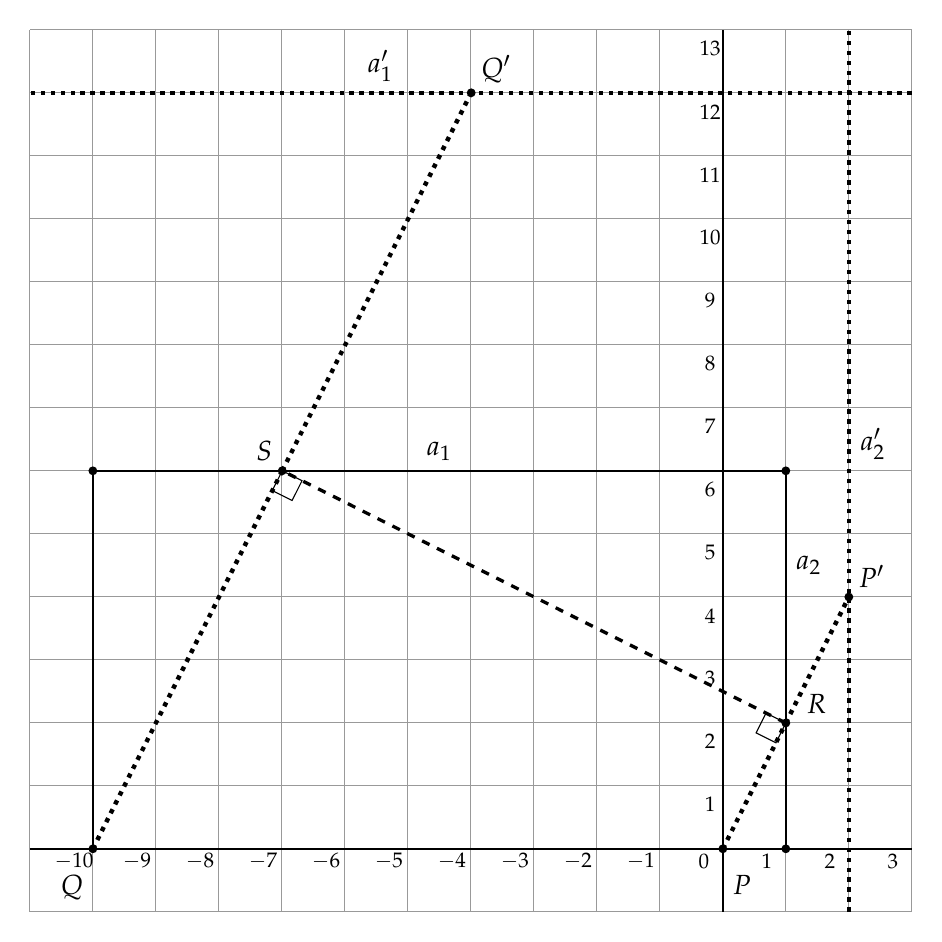
\begin{tikzpicture}[scale=.8]
% Draw help lines and axes
\draw[step=10mm,white!60!black] (-11,-1) grid (3,13);
\draw[thick] (-11,0) -- (3,0);
\draw[thick] (0,-1) -- (0,13);
\foreach \x in {-10,...,3}
  \node at (\x-.3,-.2) {\sm{\x}};
\foreach \y in {1,...,13}
  \node at (-.2,\y-.3) {\sm{\y}};
  
% Draw first path with five points
\coordinate (A) at (0,0);
\coordinate (B) at (1,0);
\coordinate (C) at (1,6);
\coordinate (D) at (-10,6);
\coordinate (E) at (-10,0);
\foreach \x in {A,B,C,D,E}
  \fill (\x) circle(2pt);
\node[below right,yshift=-6pt] at (A) {$P$};
\node[below left,yshift=-6pt] at (E) {$Q$};

\draw[thick] (A) -- (B);
\draw[thick,name path=bc] (B) -- node[right,near end] {$a_2$} (C);
\draw[thick,name path=cd] (C) -- node[above] {$a_1$} (D);
\draw[thick,name path=de] (D) -- (E);

% Draw parallel lines
\draw[ultra thick,dotted,name path=bpcp] ($(B)+(1,-1)$) --
  node[above right] {$a_2'$}
  ($(C)+(1,7)$);
\draw[ultra thick,dotted,name path=cpdp] ($(C)+(2,6)$) -- 
  node[above left,xshift=-24pt] {$a_1'$} 
  ($(D)+(-1,6)$);

% Draw first segment of second path
\path[name path=a2] (A) -- +(63.4:4);
\path [name intersections = {of = a2 and bc, by = {A2}}];
\draw[ultra thick,dotted] (A) -- (A2);
\fill (A2) circle(2pt) node[above right,xshift=4pt] {$R$};
\draw[rotate=153.4] (A2) rectangle +(10pt,10pt);

% Draw second segment of second path
\path[name path=b2] (A2) -- +(153.4:10);
\path [name intersections = {of = b2 and cd, by = {B2}}];
\fill (B2) circle(2pt) node[above left]  {$S$};
\draw[very thick,dashed] (A2) -- (B2);
\draw[rotate=243.4] (B2) rectangle +(10pt,10pt);

% Draw third segment of second path
\draw[ultra thick,dotted] (B2) -- (E);

% Locate reflections on parallel lines and draw lines
\coordinate (PP) at ($(A2)+(1,2)$);
\fill (PP) circle(2pt) node[above right] {$P'$};
\draw[ultra thick,dotted] (A2) -- (PP);

\coordinate (QP) at ($(B2)+(3,6)$);
\fill (QP) circle(2pt) node[above right] {$Q'$};
\draw[ultra thick,dotted] (B2) -- (QP);
\end{tikzpicture}
\end{center}


A line $a_2'$ is drawn so that it is parallel to $a_2$ and the same distance from $a_2$ as $a_2$ is from $P$. Similarly, line $a_1'$ is drawn so that it is parallel to $a_1$ and the same distance from $a_1$ as $a_1$ is from $Q$. Apply Axiom~6 to simultaneously place $P$ at $P'$ on $a_2'$ and to place $Q$ at $Q'$ on $a_1'$. The fold $\overline{RS}$ is the perpendicular bisector of the lines $\overline{PP'}$ and $\overline{QQ'}$; therefore, the angles at $R$ and $S$ are right angles as required.

\newpage

Let us try the Beloch fold on the polynomial $x^3-3x^2-3x+1$ from Section~\ref{s.negative}. $a_2$ is the vertical line line of length $3$ and its parallel line $a_2'$ is $x=2$. $a_1$ is the horizontal line segment of length $3$ and its parallel line $a_1'$ is $y=-2$. The fold $RS$ is the perpendicular bisector of both $\overline{PP'}$ and $\overline{QQ'}$. The line $\overline{PRSQ}$ is the same as the second path in Section~\ref{s.negative}.

\begin{center}
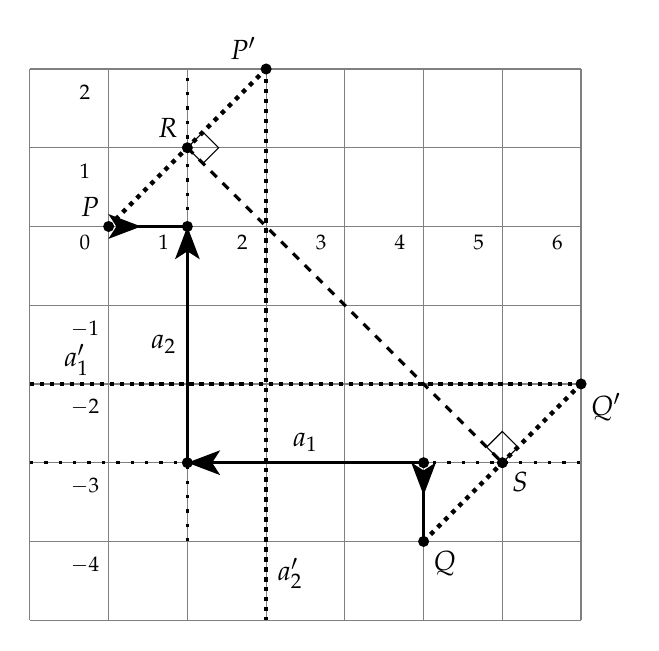
\begin{tikzpicture}[scale=1]
% Draw help lines and axes
\draw[step=10mm,white!50!black] (-1,-5) grid (6,2);
\foreach \x in {0,...,6}
  \node at (\x-.3,-.2) {\sm{\x}};
\foreach \y in {-4,...,-1}
  \node at (-.3,\y-.3) {\sm{\y}};
\foreach \y in {1,...,2}
  \node at (-.3,\y-.3) {\sm{\y}};

% Draw first path
\coordinate (A) at (0,0);
\coordinate (B) at (1,0);
\coordinate (C) at (1,-3);
\coordinate (D) at (4,-3);
\coordinate (E) at (4,-4);
\node[above left] at (A) {$P$};
\node[below right] at (E) {$Q$};
\foreach \x in {A,B,C,D,E}
  \fill (\x) circle(2pt);

\draw[very thick,{Stealth[scale=1.4,inset=2pt,reversed]}-] (A) --
  (B);
\draw[very thick,{Stealth[scale=1.4,inset=2pt]}-,name path=bc] (B) -- 
  node[left] {$a_2$} (C);
\draw[very thick,{Stealth[scale=1.4,inset=2pt]}-,name path=cd] (C) --
  node[above] {$a_1$}(D);
\draw[very thick,{Stealth[scale=1.4,inset=2pt,reversed]}-,name path=de] (D) --
 (E);

% Draw extensions of first path
\draw[very thick,loosely dotted,name path=b] (1,-4) -- (1,2);
\draw[very thick,loosely dotted,name path=c] (-1,-3) -- (6,-3);

% Draw reflected points
\coordinate (PP) at (2,2);
\coordinate (QP) at (6,-2);
\fill (PP) circle(2pt) node[above left] {$P'$};
\fill (QP) circle(2pt) node[below right] {$Q'$};

% Midpoints of bisected lines
\coordinate (R) at (1,1);
\coordinate (S) at (5,-3);
\fill (R) circle(2pt) node[above left] {$R$};
\fill (S) circle(2pt) node[below right] {$S$};

% Draw reflected lines
\draw[ultra thick,dotted] ($(B)+(1,2)$) --
  node[right,very near end,yshift=-8pt] {$a_2'$} ($(C)+(1,-2)$);
\draw[ultra thick,dotted] ($(C)+(-2,1)$) --
  node[above,very near start,xshift=-8pt,yshift=-1pt] {$a_1'$} ($(D)+(2,1)$);
\draw[ultra thick,dotted] (A) -- (PP);
\draw[ultra thick,dotted] (E) -- (QP);

% Draw fold
\draw[very thick,dashed] (R) -- (S);
\draw[rotate=-45] (R) rectangle +(8pt,8pt);
\draw[rotate=45] (S) rectangle +(8pt,8pt);
\end{tikzpicture}
\end{center}

\newpage

\section{The Beloch square}\label{s.beloch-square}

This construction can be expressed in terms of a \emph{Beloch square}: Given two points $P,Q$ and two lines $a_2,a_1$, construct a square $\overline{ARSB}$, such that:
\begin{itemize}
\item One side is $\overline{RS}$ where $R$ lies on $a_2$ and $S$ lies on $a_1$;
\item $P$ lies on $\overline{RA}$ and $Q$ lies on $\overline{SB}$.
\end{itemize}
The following diagram extends the construction for $x^3+6x^2+11x+6$ to show the Beloch square. The length of $RS$ is $\sqrt{80}=4\sqrt{5}\approx 8.94$. We can construct the square by adding three sides of this length.
\begin{center}
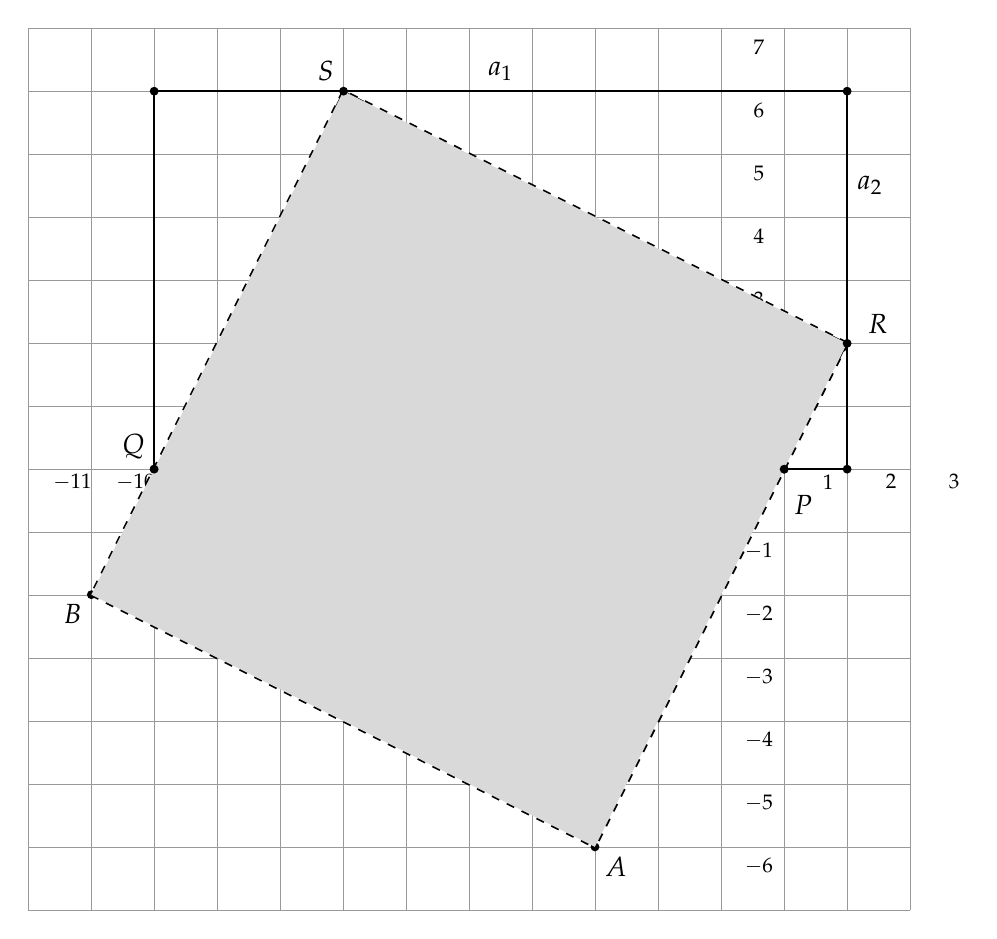
\begin{tikzpicture}[scale=.8]
% Draw help lines and axes
\draw[step=10mm,white!60!black] (-12,-7) grid (2,7);
%\draw[thick] (-12,0) -- (2,0);
%\draw[thick] (0,-7) -- (0,7);
\foreach \x in {-11,...,3}
  \node at (\x-.3,-.2) {\sm{\x}};
\foreach \y in {1,...,7}
  \node at (-.4,\y-.3) {\sm{\y}};
\foreach \y in {-6,...,-1}
  \node at (-.4,\y-.3) {\sm{\y}};

% Draw first path
\coordinate (A) at (0,0);
\coordinate (B) at (1,0);
\coordinate (C) at (1,6);
\coordinate (D) at (-10,6);
\coordinate (E) at (-10,0);
\foreach \x in {A,B,C,D,E}
  \fill (\x) circle(2pt);
\draw[thick] (A) -- (B);
\draw[thick,name path=bc] (B) -- node[right,near end] {$a_2$} (C);
\draw[thick,name path=cd] (C) -- node[above] {$a_1$} (D);
\draw[thick,name path=de] (D) -- (E);

% Find first segment of second path
\path[name path=a2] (A) -- +(63.4:4);
\path [name intersections = {of = a2 and bc, by = {A2}}];
\draw[rotate=153.4] (A2) rectangle +(10pt,10pt);

% Draw second segment of second path
\path[name path=b2] (A2) -- +(153.4:10);
\path [name intersections = {of = b2 and cd, by = {B2}}];
\draw[very thick,dashed] (A2) -- (B2);
\draw[rotate=243.4] (B2) rectangle +(10pt,10pt);

% Draw square
\draw[very thick,dashed] (B2) -- +(243.4:8.94) coordinate (AB);
\draw[very thick,dashed] (A2) -- +(243.4:8.94) coordinate (BB);
\fill (AB) circle (2pt) node[below left] {$B$};
\fill (BB) circle (2pt) node[below right] {$A$};
\draw[very thick,dashed] (AB) -- (BB);

\path[fill=white!85!black,rotate=-26.6] (AB) rectangle +(8.94,8.94);

% Draw labels of points
\fill (A2) circle(2pt) node[above right,xshift=4pt] {$R$};
\fill (B2) circle(2pt) node[above left]  {$S$};
\fill (A)  circle(2pt) node[below right,yshift=-6pt]  {$P$};
\fill (E)  circle(2pt) node[above left]  {$Q$};
\end{tikzpicture}
\end{center}

\newpage

\bibliographystyle{plain}
\bibliography{lill}

\end{document}
